\section{Integrating threads}
\label{sec:babythreads}
After familiarising myself with the VSL codebase I tried to implement the simplest form of
multi-threading and test out how the language would behave. I added a new function called \verb|thread|
to VSL which takes a piece of code as an argument, starts a new thread and joins again with
the main thread. Once implemented, I could run the first and simplest unit test for ParVSL:

\begin{verbatim}
> (dotimes (i 4) (thread '(print "Hello World")))
"Hello World"
"Hello World"
"Value: Hello Worln"Hello Woird"
ld"
\end{verbatim}

We can immediately observe the effects of parallelism in action. The interpreter is not thread-safe and data races
on global variables (including printing to the same stream) lead to undefined behaviour. Although printing
is possible, most other functions would fail. The spawned threads can only handle strings
and will crash on handling numbers or symbols, or when trying to allocate anything.
There is no inter-thread communication or exception safety, and any garbage collection would produce a segmentation
fault. To be able to write a more complicated test, I need to make changes in all areas of the interpreter.

To manage the threads, I made further use of the C++11 standard library. I devised a global hashmap storing
all the running threads. Creating and joining a thread is done under a mutex lock. Each thread is assigned its own unique
identifier, which is returned to the user. Subsequently, the user can then use the identifier to join the thread.

\section{Memory allocation}
\label{sec:malloc}
\label{sec:storage}

I wanted to allow multiple threads in parallel without affecting the performance
of allocations. To do this I had to use a lock-free approach. As such, I further
split the memory into regions, which I call \emph{segments}. A segment is a thread-local region
for allocation on the heap (see figure \ref{fig:parvslalloc}).

Just like before, memory is allocated to the segments in a continuous
fashion. A pointer indicates the start of the non-allocated part of the segment
(the \emph{segment fringe}), while another tells us the end of the segment
(the \emph{segment limit}).

\begin{figure}[H]
  \centering
  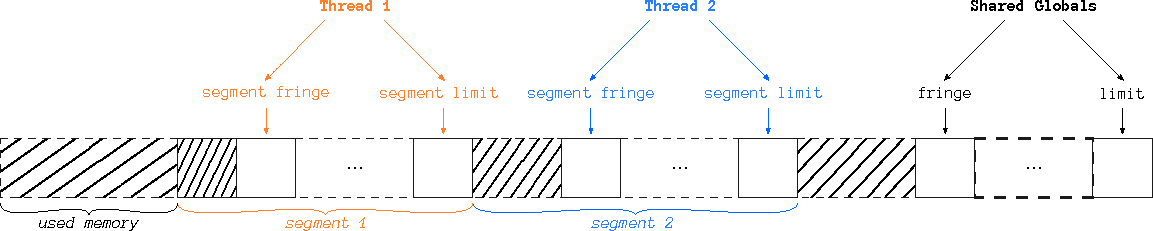
\includegraphics[width=1\linewidth]{parvslalloc.pdf}
  \caption{Memory allocations in ParVSL}
  \label{fig:parvslalloc}
\end{figure}

Now, contention is reduced to getting a new segment. Each thread only allocates within
its own segment, so allocations do not require any synchronisation, and they still only
require incrementing one variable in most cases. If the requested allocation would bring
the segment fringe over the segment limit, then the current segment is \emph{sealed} and a new one is
requested.

I carefully modified all the areas where allocations are performed to use the segment fringe
instead of the global fringe. The global fringe is only moved to assign a new segment. Writes
to the global fringe are executed under a mutex lock, while the segment fringe is a thread local
variable accessed without any locks. If the requested memory is larger than the segment size
(e.g. a large string or number), it is allocated outside any segment, using the global fringe.

There is a trade-off involved when choosing the segment size. If the size is too small,
there will be a lot of contention on requesting segments, leading back to the original
problem of locking on every allocation. If the segment size is too large, there is a risk
of threads holding large amounts of memory without using it and causing internal fragmentation and
early garbage collection cycles. This is because reclaiming memory is requested when a new segment cannot be created,
regardless of how much free space there is in existing segments. While the trade-off depends on the
total memory, I have found a good compromise for segments of a few kilobytes each.

\section{Garbage collection}
\label{sec:gc}
The garbage collector has to account for the state of all threads. These threads have to be synchronised
and in a \emph{safe} state to initiate the GC. They must also be included in the calculation of the root set.

I store all the thread-local information required for synchronisation in a class called \verb|Thread_data|. This
class is populated when a thread is started and updated before and after a GC cycle. All threads register
themselves in a global thread table at start-up. The thread starting the GC can use this table to check the status
of the other threads.

Each thread will have its own stack, so I had to modify the code to scan all the stacks before garbage
collection. This is one reason I had to pause work on all threads for GC. If I didn't it would be possible
for a thread to add references to the heap on its stack after those locations were marked safe to delete,
causing corruption.

When a thread is initialised, I save its own stack base in \verb|Thread_data|, and then also save its stack head
when it is paused to wait for GC. All these stack ranges are scanned before I start garbage collection, as shown
in \ref{code:parstackscan}.

\begin{code}
\begin{minted}[breaklines,mathescape]{c++}
void garbage_collection() {
  for (auto thread: thread_table)
    // scan the stack from its head to base
    for (uintptr_t s = thread.c_stack_head;
                   s < thread.c_stack_base;
                   s += sizeof(LispObject))
      if (in_heap(s)) { // check if s points to the virtual heap
        set_pinned(s); // found an ambiguous root
      }
  ...
}
\end{minted}
\caption{Scan the stack of each thread for pinned items before GC.}
\label{code:parstackscan}
\end{code}

\subsection{Garbage collection locks and safety}
\label{sec:gclock}
The thread initiating garbage collection must wait for all
threads to be ready. Similarly, to prevent starvation, all threads must regularly check
whether a garbage collection cycle was initiated and make themselves safe.

The first idea I had was to trap all calls to allocate memory and check whether garbage collection is needed.
To do this, I could simply reset all thread segments. Threads would need to allocate eventually and
would request a new segment, at which point they would need to call the GC. However, this solution is incomplete:
a thread might be busy for a long time without needing to allocate. This would cause all other
threads to be idle waiting for it to finish.

A bigger issue was the risk of deadlocks. In figure \ref{fig:gcdeadlock}, thread 2 for thread 1 to release
but thread 1 was paused waiting for the GC, causing a deadlock. Similarly, any effectful computation,
like waiting for user input will prevent the collection from starting.

\begin{figure}[H]
  \centering
  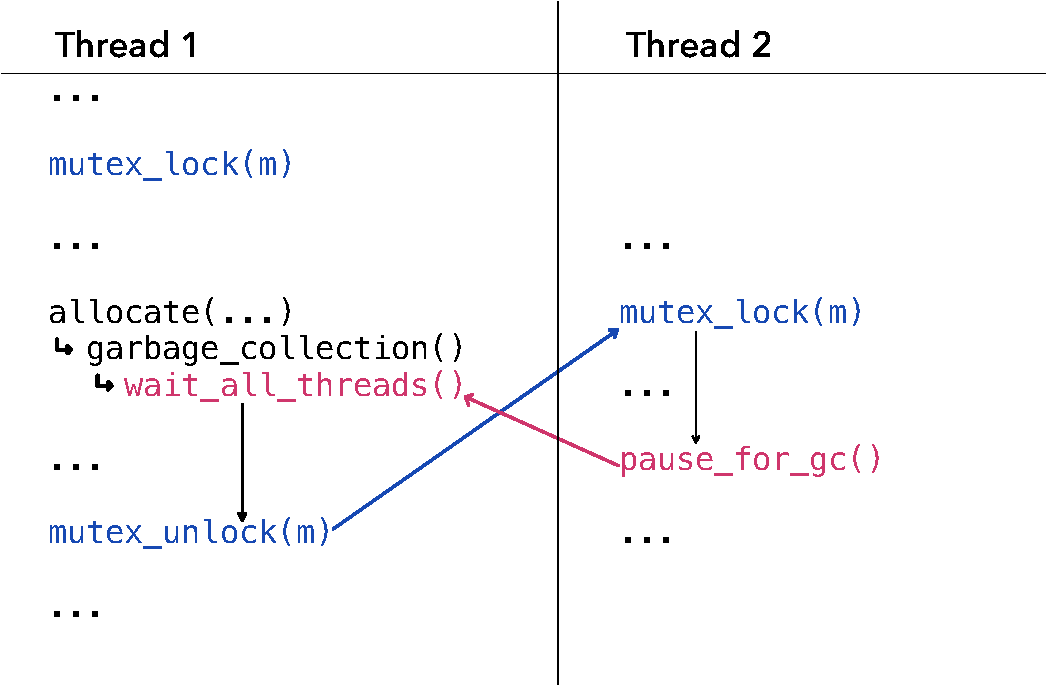
\includegraphics[width=0.8\linewidth]{gcdeadlock.pdf}
  \caption{Possible deadlock when starting garbage collection}
  \label{fig:gcdeadlock}
\end{figure}

I implemented three mechanisms
for a thread to check for garbage collection. The first one is when it tries to allocate. Then, it
polls the global flag in the interpreter, so that time-consuming loops which do not allocate do not
delay the garbage collector for too long. Finall

There are three scenarios in which a thread should check for GC. The first one is when it tries to allocate.
Then, it should poll a global flag in the interpreter, so that time-consuming loops which do not allocate do not
delay the garbage collector for too long. Finally, it must handle any blocking operation, especially
when it depends on a signal from another thread (as in \ref{fig:gcdeadlock}).

I created two classes to help me synchronise threads for GC and handle all the scenarios above:
\verb|Gc_guard| and \verb|Gc_lock|.
To begin with, I used the following shared global state:
\begin{code}
\begin{minted}[breaklines,mathescape]{c++}
  std::atomic_int num_threads(0);

  // number of threads ready for GC
  std::atomic_int safe_threads(0);

  // to wait for all threads to be GC-safe
  std::condition_variable gc_wait_cv;

  // to notify all threads that GC is completed
  std::condition_variable gc_done_cv;

  // flag indicating gc is running (or pending)
  std::atomic_bool gc_on(false);
\end{minted}
\end{code}

To deal with the issue of blocking calls, I defined another state threads can be in: \emph{safe for GC}. A thread
is in a safe state if it has saved all the information the garbage collector needs to begin (e.g. stack base
and stack head) and guarantees not to run any code that invalidates the garbage collection. Threads go into a safe
state whenever they get paused for GC. However, they can also be in safe state when waiting for a blocking call.

The \verb|Gc_guard| class handles both scenarios.
It has a constructor and a destructor and is a way for the thread to promise it is in a safe state.

\begin{code}
\begin{minted}[breaklines,mathescape]{c++}
class Gc_guard {
  // Global mutex shared by Gc_guard instance.
  static std::mutex gc_guard_mutex;

  Gc_guard() {
    td.c_stack_head = approximate_stack_pointer();

    // This thread is now safe for GC.
    safe_threads += 1;

    // Notify the thread waiting for garbage collection.
    gc_wait_cv.notify_one();
  }

  ~Gc_guard() {
    std::unique_lock<std::mutex> lock(gc_guard_mutex);

    // Wait until GC is done.
    gc_done_cv.wait(lock, []() { return !gc_on; });

    // Thread is not longer safe for GC.
    safe_threads -= 1;

    // Thread stack head will be invalidated when execution resumes.
    thread_data.c_stack_head = nullptr;
  }
};
\end{minted}
\caption{\texttt{Gc\_guard} makes a thread safe for GC.}
\label{code:gc-guard}
\end{code}

The \verb|Gc_guard| is designed to be used before any blocking call. For example,
to fix the issue in figure \ref{fig:gcdeadlock}, we simply need to modify the
code in thread 2 as follows:

\begin{code}
\begin{minted}[breaklines,mathescape]{c++}
...
{
  Gc_guard gc_guard; // thread is now safe for GC
  mutex_lock(m); // this operation may block.

  // Gc_guard destructor will block here until GC is completed.
}
...
\end{minted}
\end{code}

The \texttt{Gc\_guard} class is accompanied by \texttt{Gc\_lock}. A thread trying to initiate the GC has to
acquire a \texttt{Gc\_lock}. This lock makes further use of a mutex lock for mutual exclusion.
Additionally, it waits until all threads are in a safe state.

\begin{code}
\begin{minted}[breaklines,mathescape]{c++}
class Gc_lock {
  // Global lock shared by Gc_lock instances.
  static std::mutex gc_lock_mutex;

  // Prevents other threads from acquiring the Gc_lock.
  std::unique_lock<std::mutex> lock;

  // The GC thread needs to be in a safe state as well.
  Gc_guard gc_guard;

  // Initialise the lock and guard before Gc_lock is constructed.
  Gc_lock() : lock(gc_lock_mutex), gc_guard() {
    gc_on = true;

    // Wait until all threads are in a safe state.
    gc_wait_cv.wait(lock, []() {
      return paused_threads == num_threads;
    });
  }

  ~Gc_lock() {
    gc_on = false;

    // Notify all threads that GC is over.
    gc_done_cv.notify_all();
  }
};
\end{minted}
\caption{Garbage collection must be done under the \texttt{Gc\_lock}.}
\label{code:gc-lock}
\end{code}

\section{Lock-free hashtable for symbol lookup}
\label{sec:hashtable}
Just like allocations are a critical region of code in VSL, so are symbol lookups.
Every occurrence of a symbol must be looked up in the symbol table. If the symbol does
not exist, it will be created. Multiple threads looking up symbols will cause contention.
If two threads try to allocate the same symbol name at the same time, they will invalidate
the table.

As before, the na\"ive solution would be to implement a mutex lock on the entire
lookup function.

To improve on that I tried to use a reader-writer lock. Reader-writer locks allow grant access
to either a single writing thread, or all the reading threads. This would allow multiple
threads to lookup symbols at the same time. However, as soon as one one thread has to create a
symbol, all the readers have to wait for it to finish.

Moreover, the lookup function is two-step: first it tries to find a symbol, then it creates one
if it did not find any. In the case of two threads looking up the same symbol, it is possible for
both of them to end try to create it at the same time. The reader-writer lock would not prevent this.
It serialises the writes, so it does prevent undefined behaviour in C++, however it may
still create the same symbol twice. The pointer to the symbol that the first thread returned from the function
would become invalid.

I have found a third approach, based on the Compare-And-Swap (CAS) instruction which solves the issue
above, while also providing a lock-free implementation. The symbol lookup table is currently implemented
as a static array of linked lists. VSL never erases symbols, which made the lock-free implementation easier.

\begin{code}
\begin{minted}[breaklines,mathescape]{c++}
std::atomic<LispObject> symbol_table[TABLE_SIZE];

LispObject lookup(std::string name) {
  size_t loc = hash(name) % SYMBOLS_SIZE;

  LispObject bucket = symbols[loc].load(std::memory_order_acquire);

  while (bucket != nil) {
    LispObject s = head(bucket); // first list element

    if (symbol_name(s) == name) {
      // found the symbol
      return s;
    }

    bucket = tail(bucket); // rest of the list
  }

  LispObject s = allocate_symbol(name);

  LispObject new_bucket = cons(s, bucket);

  while (!symbols[loc].compare_exchange_strong(
      bucket, new_bucket, std::memory_order_acquire_release))
  {
    // search for stored value
    LispObject old_bucket = bucket;
    bucket = symbols[loc].load(std::memory_order_acquire);

    for (LispObject s; s != old_bucket; s = tail(s)) {
      if (symbol_name(s) == name) {
        // Another thread created the symbol. Use that.
        return s;
      }
    }

    // Make sure we don't discard new symbols inserted by other threads.
    new_bucket = cons(s, bucket);
  }

  return s;
}
\end{minted}
\caption{Lock-free symbol hashtable look up implementation}
\label{code:lockfree}
\end{code}

This approach adds no penalty to single-threaded
code. For comparison, I also implemented the mutex lock approach and tested
them on building REDUCE (single-threaded). Table \ref{tab:lockfree} shows that the mutex
version is noticeably slower, while the lock-free takes the same amount of time.

\begin{table}[H]
  \centering
  \begin{tabular}{lr}
                               & Time \\
  \hline
  VSL                          & 1m55s \\
  ParVSL with mutex lookup     & 2m10s \\
  ParVSL with lock-free lookup & 1m55s \\
  ParVSL with std::string      & 2m04s
  \end{tabular}
  \caption{Symbol lookup effects on building REDUCE}
  \label{tab:lockfree}
\end{table}

\subsection{Impact of C++ \texttt{std::string} on performance}

While modifying this code, I saw the opportunity to change C-style string to C++
standard library ones. The lookup function, for example, actually takes a char array
pointer and the string length as separate arguments. I even identified a bug
in VSL where the wrong length was passed as a hard-coded number, and it prompted
me to use the more modern \verb|std::string| class. Surprisingly, this change alone
slowed down ParVSL, as can be seen in the last row of Table \ref{tab:lockfree}.
I made sure no more extra copying or construction of these strings was done than
necessary. I reverted my change in this case, but I note it as an interesting example
of the trade-off C++ features can bring.

\section{Symbol access}
\label{sec:symbols}

All named objects in the lifecycle of the program are \emph{symbols}. All global and local variables, including
special ones (like \texttt{true} or \texttt{nil}) and function arguments are symbols. A global hash-table keeps track of
all symbols. This means each name can only be in use in one place at a time.

Lisp is a language with dynamic scope. This has many implications for the interpreter. The following
fragment of code is an example of this behaviour:
\begin{verbatim}
let f x = x + y in
let g () =
  let y = 3 in
  f 2
in
g ()
\end{verbatim}

The above example will not compile in any statically scoped languages such as OCaml or C++
because the variable \verb|y| is not defined in the scope of \verb|f|.
Most dynamic languages, even weakly typed ones, like Javascript or Python, will consider the equivalent
code valid, but will encounter a runtime error because \verb|y| is not defined.
Lisp, and VSL in particular, has a much looser concept of scope.
In the example above, \verb|y| is defined before the call of \verb|f| and will remain defined until the
call to \verb|g| returns.

\emph{Shallow binding} is the mechanism through which this is achieved. Each symbol is mapped to a single value.
When a variable name is bound, e.g. as a function parameter name during a function call or through a
\texttt{let} statement, its old value is stored by the interpreter and replaced with the new value. At the end of the binding,
the old value is restored. The main advantage of this method is performance. Old values can simply be saved
on the stack:
\begin{verbatim}
let varName = expr1 in expr2
\end{verbatim}

can be implemented as:

\begin{code}
\begin{minted}[breaklines,mathescape]{c++}
void implement_let(string varName, LispObject expr1, LispObject expr2) {
  LispObject symbol = lookup_symbol(varName);
  LispObject oldVal = value(symbol); // store the old value
  value(symbol) = eval(expr1);       // replace with new value
  eval(expr2);                       // evaluate the rest of the code
  value(symbol) = oldVal;            // restore old value
}
\end{minted}
\caption{Implementation of \texttt{let} in VSL.}
\label{code:let-vsl}
\end{code}

This mechanism was not designed with concurrency in mind, and is not thread-safe.
Many variable names are reused multiple times in a program (e.g. \texttt{i, j, count}, etc).
Multiple threads binding the same variable will override each other's values.

I wanted to fix this while keeping the same dynamic scoping semantics for backward compatibility.
One option was to implement a form of deep binding with association lists storing local values,
yet performance was a concern. While shallow binding has a constant factor, deep binding requires
an associative data structure which would add non-negligible overheads to a critical area of the
interpreter.

My approach was to allocate thread-local storage for symbols.
Global symbols were unaffected, because rebinding them is illegal in the language.
However, for non-globals I used a thread-local array to store the real value, and had the global storage
location point to the array location. A globally unique array index is reserved for each local symbol.
All threads reserve that location within their local arrays for the symbol.

\begin{minted}[breaklines,mathescape]{c++}
thread_local vector locals;
vector shared_fluids;

LispObject par_value(LispObject symbol) {
  // [value] returns the symbol's global value
  LispObject val = value(symbol);

  if (is_global(symbol))
    return val; // global symbols remain unaffected

  int loc = to_int(val); // val is a location

  if (is_fluid(symbol) and locals[loc] == undefined)
    // No local value for this fluid. Return the global one.
    return shared_fluids[loc];

  // get the thread-local value at that location
  return locals[loc];
}
\end{minted}

I carefully replaced all calls to \texttt{value} to use \texttt{par\_value} instead.
Now, multiple threads accessing the same symbol can do so safely,
as they will each access their own versions. This eliminates data races entirely,
and shallow binding is unaffected.

\begin{figure}[H]
  \centering
  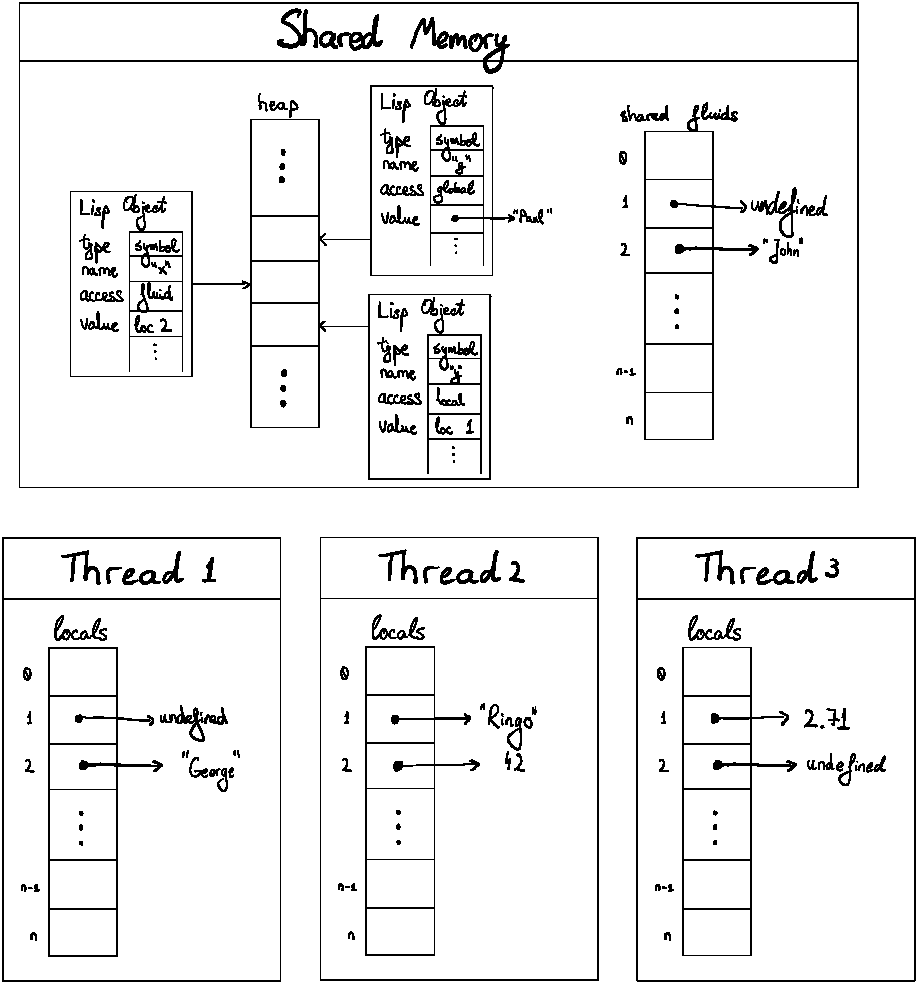
\includegraphics[width=0.9\linewidth]{symbols.pdf}
  \caption{Storage of symbols in ParVSL}
  \label{fig:symbols}
\end{figure}

In figure \ref{fig:symbols} I show a full example of how symbols are stored. The first symbol is \texttt{g}, which
is a \emph{global} symbol. Its value is stored directly in the global heap (like in the original VSL). The symbol \texttt{x}
is \emph{fluid}. Its heap value simply indicates a location (\texttt{loc 2}). We use the index to find the actual value
in thread-local storage. Threads 1 stores the string \texttt{"George"} while thread 2 stores the integer \texttt{42}.
Thread 3 has not bound any local value to the symbol so it is \texttt{undefined}. However, it can still access the
global value in \verb|shared_fluids|, the string \verb|"John"|. Finally, symbol \verb|y| is \emph{local}. It is
undefined in \verb|shared_fluids| but otherwise behaves the same as \verb|x|, storing its thread-local values at
index \verb|1|.

I redesigned shallow binding to use a RAII style class, called \verb|Shallow_bind| which deals with all the changes
described above, while providing more safety guarantees, thus leading to more robust code. It checks if the symbol is global and prevents binding,
it handles thread-local storage and it always restores the old value correctly in its destructor, including the
case of exceptions. Previous code spent time testing error flags, manually restoring the old value in every place.
For example, the code in listing \ref{code:let-vsl} was rewritten as:
\begin{code}
\begin{minted}[breaklines,mathescape]{c++}
void implement_let(string varName, LispObject expr1, LispObject expr2) {
  LispObject symbol = lookup_symbol(varName);
  Shallow_bind bind_var{symbol, eval(expr1)};
  eval(expr2); // evaluate the rest of the code
}
\end{minted}
  \caption{Implementation of \texttt{let} in ParVSL.}
  \label{code:let-parvsl}
\end{code}

\section{Data races in the interpreter}
\label{sec:datarace}

Running VSL in parallel involves, in effect, running an interpreter in each thread. The spawned threads do not
run a read-eval-print loop, instead they run a computation, save the result, then terminate. However,
in ParVSL I allow these threads to execute any code the main thread can, with no restriction. This means
all threads can use and modify global state and interact with standard input, output and files and
thus can conflict with each other.

There are plenty of global variables holding state in VSL. I discovered which ones represented local
state.
One example is \verb|unwind_flag|, which is heavily used for Lisp control flow. Among other uses, it is
mutated to indicate an exception, to implement \verb|goto| and \verb|return| instructions,
as well as to indicate early program exit,
among other uses. Each thread needs its own version of this global flag, otherwise they will mess with each
other's control flow, so I made it \emph{thread-local}.

A third case is file handling. Global variables indicate which file is in use, and hold buffers for reading
and writing. Again, I had to make all these thread-local. On the other hand, there are other variables holding
truly global information, like file handles. At one point I was over-zealous in
my modifications and made a variable thread-local which should have stayed global. Although tt looked as if it indicated
the direction of the current file, it turned out to be a bitmap of all the files in the system. The fact
that VSL makes creative uses of integers for optimisation reasons effectively hides information from the type system.
After a significant time spent debugging, I realised that the variable was used differently and the solution became apparent.
I also modified the variable to use a proper \emph{bitset} data structure, enhancing readability.
As a bonus, ParVSL can now support a much larger number of open files than the 32 imposed by the size of integers.

Those globals which are not thread-local still pose the problem of data races. For instance, multiple threads
may try to read from or write to the same file. ParVSL cannot avoid contention altogether: those conflicting
operations will be serialised non-deterministically. However, it is important to prevent these data races at
the C++ level, because they cause undefined behaviour, ultimately leading to anything from spurious crashes
to more subtle data corruption.

I changed all functions for opening, closing, or altering a file to use mutex locks, with one mutex per file.
Opening and closing files are not on the critical path of the interpreter so time was less of a concern.
However, reading and writing can be part of the main loop. Many programs will run from a file, not standard input,
and it is common to print regularly to standard output or file. To manage this, I added extra per-thread buffers
to handle single character reads and writes. Then, I only synchronise threads when flushing the buffers, reducing
contention. In my testing, these changes did not slow down ParVSL in any measurable way.

\section{Threads and synchronisation in ParVSL}
\label{sec:threads}

At the start of the project I bolted on to ParVSL a small, broken, but very much useful feature to evaluate
Lisp code in a new thread, as demonstrated in section \ref{sec:babythreads}. I ran a number of small tests
and found where this functionality broke the interpreter, then reworked those parts of the Lisp system
until it successfully passed the tests. At the same time, I adapted a large suite of regression tests
from REDUCE to ensure single-threaded behaviour was unaffected and performance didn't degrade significantly.
Once I was confident that ParVSL could run multi-threaded I started implementing the extra functionality
required to make parallel programs practical.

To start a thread, the user needs to call the \verb|thread| function.
Originally, the function only took a Lisp expression as argument and evaluated it. This was highly impractical,
as the expression was passed unevaluated and data could not be passed naturally. The only way to allow
communication was to write the data into a global symbol and have the code executed access that symbol.

I changed the implementation of \verb|thread| to instead accept a function function name and the argument list
as arguments. The arguments can be local symbols, and their values will be correctly bound to parameter names
within the thread. The spawned thread then applies the function to the arguments and saves the result
before terminating. The return value of \verb|thread| is the thread id, which then has to be used to
join the thread. Calling  \verb|join_thread| on the thread id, will block until the thread has finished
executing, and retrieve the resulting value of the computation.

\begin{verbatim}
tid := thread('add, {2, 3});
result := thread_join tid;
print result;
> 5
\end{verbatim}

My implementation minimises overhead. The list of arguments is managed on the heap which is visible by all
threads, so a simple pointer is enough to pass them. Furthermore, all unjoined threads and corresponding return values
need to be tracked.
A hashmap from thread ids to return values is updated when thread execution is completed.
Consequently, when \verb|thread_join| is called this value is returned and removed from the hashmap. All threads
have unique ids for the lifetime of the program, so there are never any conflicts in the hashtable.
Starting and joining a thread are synchronised under a mutex lock to prevent data races.

I was careful to prevent the garbage collector from collecting these parameters and return values.
Starting a thread is GC-safe: garbage collection will not initiate while a new thread is starting up. This ensures
that threads are always in a safe state and registered in the thread-table correctly during garbage collection.
At that point, function parameters are tracked just like regular variables so they will be safe from GC.
However, return values are stored past the lifetime of their respective threads, so I add them
to the unambiguous root set at the beginning of garbage collection.

\subsection{Mutual exclusion and condition variables}

It is not enough for the user to be able to spawn threads. ParVSL has a shared memory model so at a minimum
it has to provide a way to mechanism for mutual exclusion. I exposed the C++ \emph{mutex locks}
with a very simple interface:

\begin{verbatim}
m := mutex();
mutex_lock(m);
mutex_unlock(m);
\end{verbatim}

The mutexes are created in C++ and stored in a lock-free hashtable, each with a unique id. I used the lock-free
hashtable implementation to allow different mutexes to be accessed in parallel. I also
make use of the \verb|Gc_guard| when \verb|mutex_lock| is called. This is to ensure that the blocking
call to lock the mutex does not cause a deadlock during garbage collection.

While ParVSL users can use mutexes to protect against data races, they may not always do so
(due to omissions or bugs). Operations such as modifying a global symbol or mutating a list in place
may still clash.
One way to ensure safety would be to lock the mutex for any such operations, but this change would add a
too much overhead to ParVSL. With this in mind, the decision was made to leave this issue as a responsibility
of the ParVSL user, since they can manage the trade-off between safety and lock usage minimisation.

The second primitive that I added was \emph{condition variables}. They provide a useful way for
threads to signal each other, enabling an efficient way to perform common parallel processes such as
waiting for a task to finish. I stored the condition variables the same way as the mutexes (i.e. in a lock-free
hashtable) and the wait operation uses the \verb|Gc_guard| to check for garbage collection.

I included a few more helpful function such as \verb|hardware_threads| to check the number of hardware
threads on the current system, \verb|yield| to allow the system to reschedule the thread, and
\verb|sleep| to pause the thread for a specified duration.

These primitives are versatile enough to enable parallel algorithms, as I will showcase in Chapter \ref{ch:evaluation}.
They can also be used to implement other common threading gadgets, such as atomics and futures
(see \ref{ssec:managethreads} and \ref{ssec:waitjob}).

\section{Saving state to disk and reloading}
\label{sec:preserve}

REDUCE has an important feature which allows the user to preserve the state to disk. A \texttt{preserve} instruction can be
used to do so, and the user is able to specify a function to run on restart. \verb|preserve| saves the entire state of the
program, including memory and symbols.

It is difficult to keep the same guarantees when multiple threads are running.
If a thread attempts to preserve while others
are running, the contents of the final image will be non-deterministic and generally undesirable,
even if all data races were resolved. At the same time, I found little benefit to implementing such
a feature, as the ability to preserve is useful in retaining the results of computations, not intermediate states.
Saving state to disk is used at the end of the program.

Once all threads are joined and there is only one thread running, all the
thread-local data can be treated as global again and stored in the same locations that
VSL uses. When restoring from an image, this data is moved back into thread-local storage. The image
format is not affected.